% Reviewer-facing replacement for the supplementary experiment section.
% Required packages: amsmath, booktabs, graphicx, and xcolor.
% Figure paths are relative to this file's directory.

\begingroup
\color{blue}

\section{Additional Numerical Results}
\label{app:additional-experiments}

This appendix reports the sensitivity analyses and stress tests supporting
Section~\ref{sec:numerical-experiments}. Unless stated otherwise, the
absolute-residual experiments use $d=10$, target coverage $0.9$, and 200
repetitions. The regression and evaluation protocol is the same as in
Section~\ref{sec:absolute-residual-experiments}: ordinary least squares is fit
on 7,200 independently drawn training observations, and coverage is evaluated
on 800 fresh test observations. The calibration sample is also independently
redrawn in every repetition, while the underlying regression coefficients are
held fixed. The CQR experiments use 30 repetitions with 2,400 training and 600
test observations per repetition; the shape-template comparison uses the same
training/test sizes and 100 repetitions. Figures show mean curves without
error bars, while the accompanying CSV files retain across-repetition standard
deviations.

\subsection{Coverage Uncertainty Audit}
\label{app:coverage-uncertainty}

We audited all 58 plotted TSCP points in the synthetic figures and the
real-data table. The corresponding nominal target lies within one
across-repetition standard deviation of every reported mean. Only four
synthetic means are below their targets: partial heteroskedasticity at
$n=500$ gives $0.8996\,(0.0164)$; capped-score CQR at $n=50$ gives
$0.8991\,(0.0457)$; $5\%$ contamination gives $0.8995\,(0.0297)$; and
Student $t_{1.5}$ noise at $n=500$ gives $0.8976\,(0.0173)$. Parentheses in
this paragraph contain one standard deviation across repetitions.

Because training, test, and calibration observations are independently
redrawn, the repetitions in the revised experiments are independent. Dividing
the preceding standard deviations by the square root of the number of
repetitions therefore gives a Monte Carlo standard error. The resulting
normal-approximation $95\%$ intervals are, respectively,
$[0.89734,0.90189]$, $[0.88271,0.91541]$, $[0.89536,0.90360]$, and
$[0.89522,0.90003]$; each contains the target $0.9$. Thus, the small displayed
shortfalls are consistent with finite Monte Carlo averaging and do not reveal
a systematic coverage defect in these experiments. The complete pointwise
check is provided in \texttt{coverage\_uncertainty\_audit.csv} and can be
reproduced with \texttt{audit\_coverage.py}.

\subsection{Dependence Strength}
\label{app:dependence-sensitivity}

We first vary the equicorrelation of the Gaussian noise over
$\rho\in\{0,0.3,0.6,0.9\}$ while retaining marginal standard deviations
$(10,9,\ldots,1)$ and a calibration size of $n=100$. Figure~\ref{fig:app-dependence}
shows that TSCP's empirical joint coverage is stable across this range:
$0.905$, $0.905$, $0.907$, and $0.908$, respectively. Its average
residual-space volume decreases from $6.37\times10^{10}$ at $\rho=0$ to
$9.47\times10^9$ at $\rho=0.9$. Point CHR and Unscaled Max also remain close
to the target. Emp. Copula improves as the correlation strengthens but remains
below the nominal level throughout the sweep. The experiment therefore does
not indicate a coverage failure of TSCP under strong equicorrelation, while
also showing that dependence materially changes region size.

\begin{figure*}[t]
  \centering
  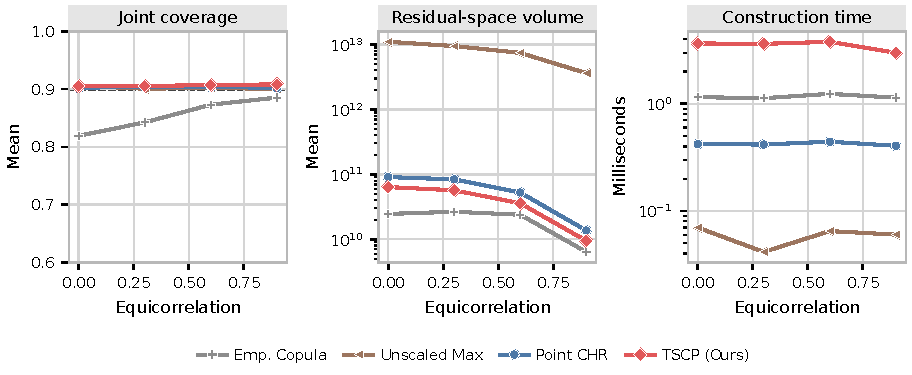
\includegraphics[width=0.92\textwidth]{figures/fig_app_dependence_sensitivity.pdf}
  \caption{Sensitivity to equicorrelated Gaussian noise at $d=10$ and
  $n=100$. The three panels report joint coverage, mean residual-space
  volume, and mean construction time. Results average 200 repetitions; the
  dashed line marks the target coverage.}
  \label{fig:app-dependence}
\end{figure*}

\subsection{Severity of Coordinate Heterogeneity}
\label{app:heterogeneity-sensitivity}

To isolate heterogeneity across outcomes, we use independent Gaussian noise
and choose ten coordinate scales geometrically spaced between $r$ and $1$,
where $r\in\{1,2,5,10,20\}$. The calibration size is fixed at $n=100$.
Figure~\ref{fig:app-heterogeneity} shows that the coverage of TSCP, Point CHR,
and Unscaled Max is essentially unchanged as $r$ grows. At $r=1$, Unscaled
Max is slightly smaller than TSCP, with mean volumes $1.43\times10^4$ and
$1.80\times10^4$. At $r=20$, their mean volumes are
$3.44\times10^{15}$ and $5.75\times10^{10}$, respectively. This widening gap
is the expected benefit of coordinate adaptation: a single maximum-residual
threshold becomes increasingly inefficient when one scale must be used for
all coordinates. Emp. Copula remains smaller but has average coverage about
$0.821$ in this experiment.

\begin{figure*}[t]
  \centering
  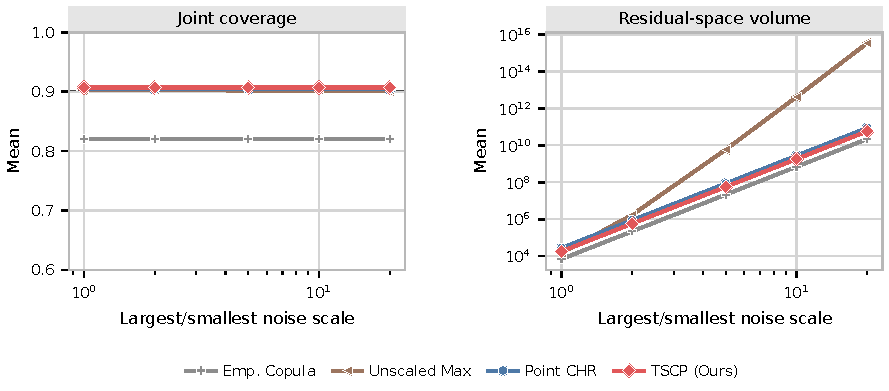
\includegraphics[width=0.84\textwidth]{figures/fig_app_heterogeneity_sweep.pdf}
  \caption{Sensitivity to the ratio between the largest and smallest outcome
  noise scales, with independent Gaussian errors and $n=100$. The scales are
  geometrically spaced, and both axes of the volume panel are logarithmic.
  Results average 200 repetitions.}
  \label{fig:app-heterogeneity}
\end{figure*}

\subsection{Target Level and Small Calibration Samples}
\label{app:alpha-small-sample}

Figure~\ref{fig:app-alpha} repeats the dependent Gaussian experiment at
nominal coverage levels $0.8$, $0.9$, and $0.95$, with $n=100$ and
$\rho=0.6$. TSCP achieves empirical coverages $0.811$, $0.907$, and $0.954$.
As expected, increasing the target level increases all region volumes. The
relative ordering is stable: TSCP is smaller than Point CHR and dramatically
smaller than Unscaled Max, while Emp. Copula is smaller but below the nominal
coverage at every displayed target.

\begin{figure*}[t]
  \centering
  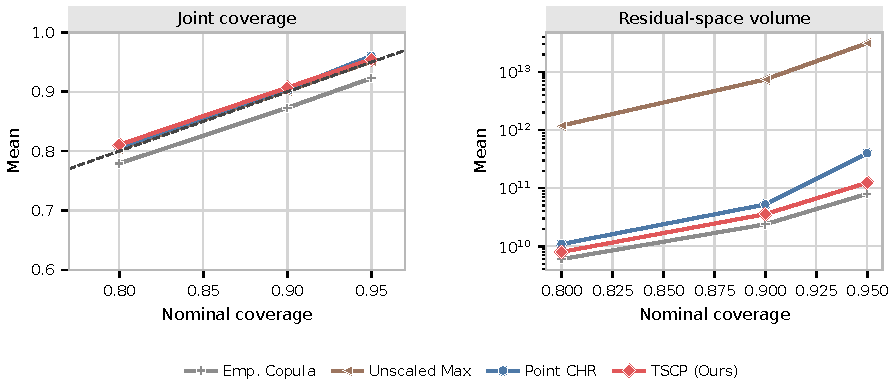
\includegraphics[width=0.84\textwidth]{figures/fig_app_alpha_sensitivity.pdf}
  \caption{Sensitivity to the nominal coverage level in the $d=10$
  equicorrelated Gaussian experiment with $n=100$ and $\rho=0.6$. The dashed
  diagonal in the left panel is exact nominal calibration. Results average
  200 repetitions.}
  \label{fig:app-alpha}
\end{figure*}

We separately examine $n\in\{10,20,30,50,100\}$ under independent Gaussian
noise. Figure~\ref{fig:app-small-calibration} distinguishes finite volumes
from the frequency of infinite output. At $n=10$, Point CHR has coverage one
and infinite volume in every repetition. This is a finite-sample quantile
effect, not evidence of a superior region: Point CHR divides the calibration
sample and its final subset is too small to supply a finite $0.9$ conformal
quantile. Point CHR is finite in all repetitions once $n\geq20$. TSCP and
Unscaled Max are finite throughout; both are conservative at the smallest
sample sizes, as expected from the discrete conformal rank. Emp. Copula
severely undercovers when $n$ is small because it estimates dependence and
calibrates on the same limited sample.

\begin{figure*}[t]
  \centering
  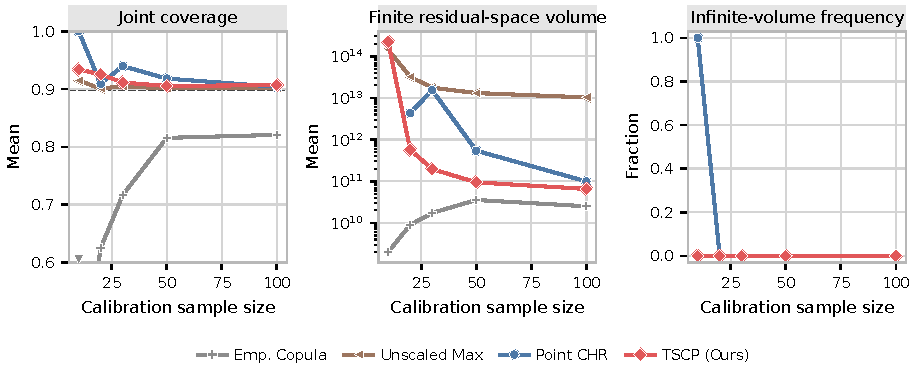
\includegraphics[width=0.92\textwidth]{figures/fig_app_small_calibration.pdf}
  \caption{Small-calibration-sample stress test with independent Gaussian
  noise and scales $(10,9,\ldots,1)$. The middle panel averages only finite
  residual-space volumes; the right panel reports the fraction of repetitions
  with infinite volume. A downward triangle at the lower plotting boundary
  marks the Emp. Copula mean below $0.6$. Results average 200 repetitions.}
  \label{fig:app-small-calibration}
\end{figure*}

\subsection{Heavy-Tailed Noise and the Role of Moment Conditions}
\label{app:heavy-tails}

The original heavy-tail experiment is reorganized in
Figure~\ref{fig:app-heavy-tails}. It uses independent Student $t$ noise with
$d=10$, a common unit scale across coordinates, and degrees of freedom
$\nu\in\{1.5,2,3\}$. The cases $\nu=1.5$ and $\nu=2$ have infinite variance
and therefore lie outside any finite-second-moment efficiency assumptions;
$\nu=3$ has finite variance but remains heavy-tailed. These results should be
read as an empirical stress test, not as an extension of the efficiency
theory to infinite-variance distributions.

TSCP remains near the target in the displayed cases. For example, at $n=30$
its coverages are $0.909$, $0.908$, and $0.912$ as $\nu$ increases, while at
$n=500$ they are $0.898$, $0.901$, and $0.900$. Efficiency is much less
stable. At $n=30$, the mean TSCP volume falls from $1.59\times10^{20}$ for
$\nu=1.5$ to $5.92\times10^{13}$ for $\nu=3$; at $n=500$, it falls from
$8.42\times10^{13}$ to $6.07\times10^7$. The explosive volumes make clear
that empirical coverage alone is not evidence of practically useful behavior
under very heavy tails.

\begin{figure*}[t]
  \centering
  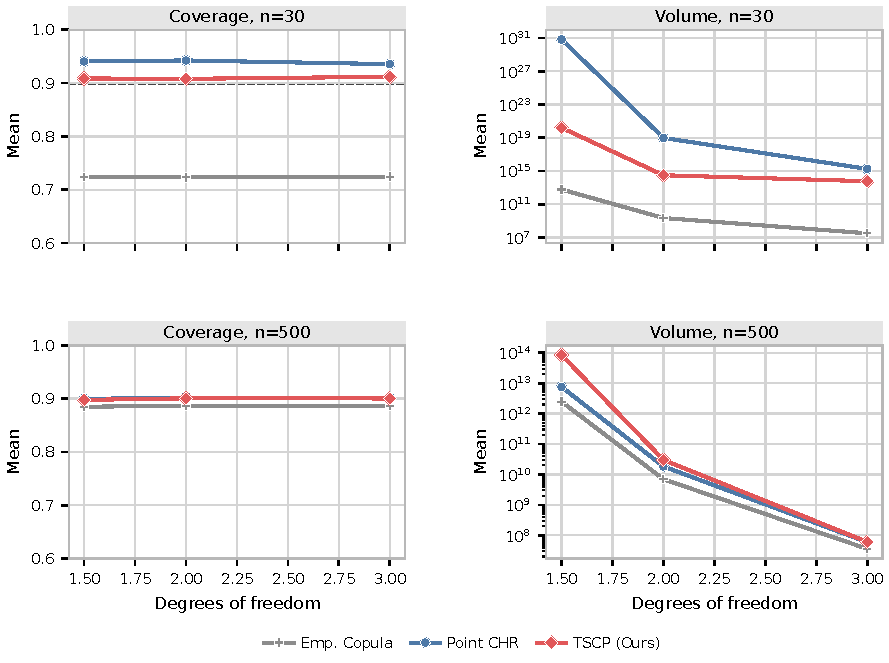
\includegraphics[width=0.86\textwidth]{figures/fig_app_heavy_tail_stress.pdf}
  \caption{Coverage and mean residual-space volume under independent,
  common-scale Student $t$ noise for $d=10$. The top row uses $n=30$
  calibration examples and the bottom row uses $n=500$. Results average 200
  repetitions; volume is shown on a logarithmic scale.}
  \label{fig:app-heavy-tails}
\end{figure*}

\subsection{Exchangeable Contamination Stress Test}
\label{app:contamination}

To test sensitivity to atypically large residuals, we contaminate the
Gaussian experiment at rates
$\varepsilon\in\{0,0.01,0.05,0.10\}$. Independently for each observation, all
ten noise coordinates are multiplied by $10$ with probability $\varepsilon$;
the same exchangeable mechanism is used for training, calibration, and test
data. The calibration size is $n=100$. We report median rather than mean
volume because the contaminated distribution produces a small number of
extreme regions.

Figure~\ref{fig:app-contamination} shows that TSCP coverage changes from
$0.904$ without contamination to $0.902$ at $10\%$ contamination, but its
median volume grows from $5.38\times10^{10}$ to $1.10\times10^{17}$. Point CHR
and Unscaled Max exhibit the same qualitative inflation, and Emp. Copula
under-covers at every contamination level. Thus, the conformal calibration is
comparatively stable in coverage, whereas the sample mean and standard
deviation used for coordinate scaling are not robust efficiency summaries.
Replacing them by robust estimators would change the construction and its
analysis, so we leave that variant for future work rather than implying a
guarantee not established here.

\begin{figure*}[t]
  \centering
  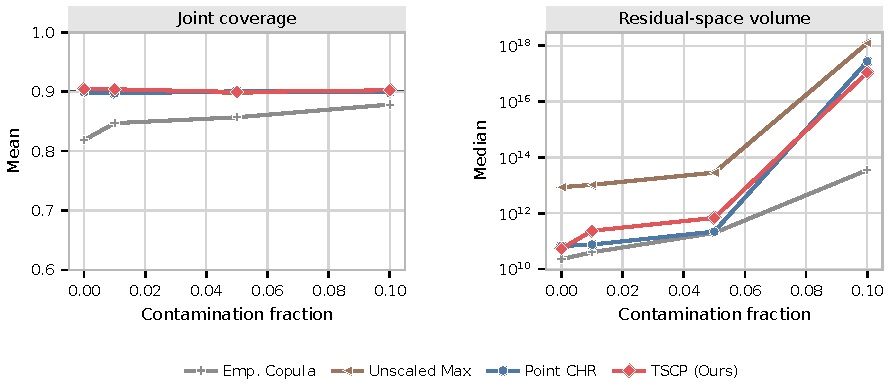
\includegraphics[width=0.84\textwidth]{figures/fig_app_contamination_stress.pdf}
  \caption{Row-wise contamination stress test with $d=10$ and $n=100$. A
  contaminated observation has every noise coordinate multiplied by $10$.
  The right panel reports median residual-space volume over 200 repetitions
  on a logarithmic scale.}
  \label{fig:app-contamination}
\end{figure*}

\subsection{Additional CQR Sensitivity Analyses}
\label{app:cqr-sensitivity}

\paragraph{Base-interval width.}
The main CQR comparison uses base-interval miscoverage $0.5$. We repeat it at
$0.3$, $0.5$, $0.7$, and $0.9$, fixing $n=100$ and final miscoverage $0.1$.
Figure~\ref{fig:app-cqr-base} shows that capped-score TSCP has empirical
coverage between $0.903$ and $0.906$ and mean outcome-space volume between
$2.80\times10^4$ and $3.77\times10^4$ across the sweep. Unscaled Max behaves
similarly, while Emp. Copula undercovers. CQHR remains close to nominal
coverage but its volume is highly sensitive to the fitted base interval in
this design. The result supports using the moderate $0.5$ base interval for
the primary comparison and cautions against drawing conclusions from one
extreme base-quantile choice.

\begin{figure*}[t]
  \centering
  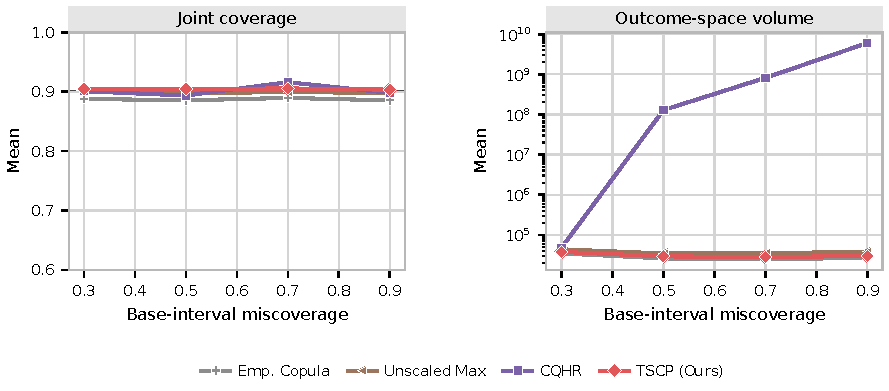
\includegraphics[width=0.84\textwidth]{figures/fig_app_cqr_base_interval.pdf}
  \caption{CQR sensitivity to the base-interval miscoverage with $d=3$,
  $n=100$, and final target coverage $0.9$. TSCP uses capped scores, CQHR uses
  its native construction, and results average 30 independent repetitions.}
  \label{fig:app-cqr-base}
\end{figure*}

\paragraph{Shifted scores.}
An alternative way to enforce nonnegativity is to replace the signed CQR score
$S_j$ by $S_j+C$, apply TSCP, and subtract $C$ from the final coordinate
adjustment. We test $C\in\{100,300,1000\}$. As shown in
Figure~\ref{fig:app-cqr-shift}, the resulting TSCP rectangle is invariant to
$C$ in this range and agrees exactly, to recorded numerical precision, with
the TSCP-GWC rectangle: the maximum coordinate-length difference is zero in
all 30 repetitions for every $C$. Consequently, this experiment does not
identify a practically meaningful shift constant and the shifted construction
does not provide a distinct local refinement. We therefore retain the capped
nonnegative score in the main text and do not recommend tuning $C$.

\begin{figure*}[t]
  \centering
  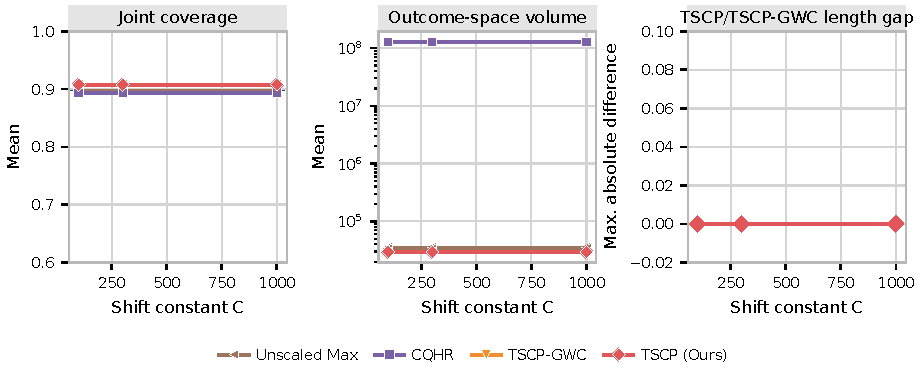
\includegraphics[width=0.92\textwidth]{figures/fig_app_cqr_shift_sensitivity.pdf}
  \caption{Sensitivity of shifted CQR scores to the additive constant $C$.
  The first two panels report coverage and mean outcome-space volume; the
  third reports the maximum coordinate-length difference between shifted TSCP
  and TSCP-GWC. Results use $d=3$, $n=100$, and 30 independent repetitions.}
  \label{fig:app-cqr-shift}
\end{figure*}

\subsection{Low-Dimensional Shape-Template Baseline}
\label{app:shape-template}

Finally, we compare with the convex shape-template approach of Tumu et
al. (2024). We use the public \texttt{conformal-region-designer} components:
a kernel density estimate on a grid of size $20$ per dimension, mean-shift
clustering, and an axis-aligned hyperrectangular template. The signed
calibration residuals are divided equally between fitting the density and
template and conformalizing its inflation. We use a score-consistent
hyperrectangle implementation and impose an aspect-ratio floor of $0.05$ when
a very small fitted cluster is degenerate along one coordinate. This detail
keeps the conformal inflation finite and is stated here because it differs
from calling the released rectangle class without modification.

The comparison uses $d=2$, independent Gaussian scales $(2,1)$, and
$n\in\{30,50,100,200\}$. Shape-template volume is divided by $2^d$ to match
the residual-space volume convention used for the symmetric rectangular
methods. Figure~\ref{fig:app-shape-template} shows broadly comparable coverage.
At $n=100$, the shape-template method has coverage $0.904$, mean normalized
volume $10.07$, and mean construction time $98.7$ milliseconds; TSCP has
coverage $0.906$, mean volume $8.04$, and mean construction time $0.80$
milliseconds. Across all displayed sample sizes, TSCP is smaller and more
than two orders of magnitude faster in this implementation.

This is deliberately a low-dimensional comparison. A Cartesian KDE grid has
$20^d$ locations and is therefore not computationally meaningful at the
$d=10$ scale of the main synthetic experiment. The experiment establishes a
comparison with a flexible convex template where the released computational
strategy is applicable; it is not evidence that either method dominates all
shape-template choices in higher dimensions.

\begin{figure*}[t]
  \centering
  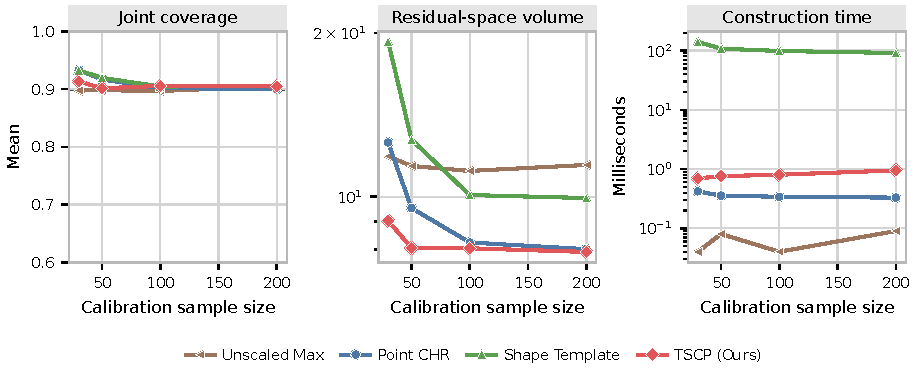
\includegraphics[width=0.92\textwidth]{figures/fig_app_shape_template_baseline.pdf}
  \caption{Comparison with a KDE/mean-shift hyperrectangular shape template
  for $d=2$ Gaussian residuals with scales $(2,1)$. Volume follows the same
  $2^{-d}$ normalization as the other residual-space experiments. Results
  average 100 independent repetitions, and runtime excludes the common
  regression fit.}
  \label{fig:app-shape-template}
\end{figure*}

\endgroup
